% "{'classe':('PSI'),'chapitre':'slci_pi','type':('td'),'titre':'Étude d\\'un automate d\\'exploration de l\\'hémostase par chronométrie', 'source':'Émilien Durif ','comp':('C1-02','C2-04'),'corrige':True}"
%\setchapterimage{bandeau}
\chapter*{TD \arabic{cptTD} \\ 
Étude d'un automate d'exploration de l'hémostase par chronométrie -- 
\ifprof Corrigé \else Sujet \fi}
\addcontentsline{toc}{section}{TD \arabic{cptTD} :
Étude d'un automate d'exploration de l'hémostase par chronométrie -- 
\ifprof Corrigé \else Sujet \fi}

\iflivret \stepcounter{cptTD} \else
\ifprof  \stepcounter{cptTD} \else \fi
\fi

\setcounter{question}{0}
\marginnote{Émilien Durif.}
\marginnote[1cm]{
\UPSTIcompetence[2]{C1-02}
\UPSTIcompetence[2]{C2-04}}

%\begin{marginfigure} [4cm]
%\centering
%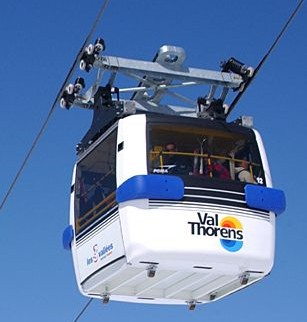
\includegraphics[width=.6\linewidth]{fig_00}
%\end{marginfigure}


\subsection*{Présentation}

La société Stago est un laboratoire pharmaceutique de l'industrie du Diagnostic In Vitro (DIV) entièrement dédiée à l'exploration de l'hémostase et de la thrombose. L'hémostase est le processus physiologique qui permet d'interrompre le saignement pour éviter l'hémorragie. L'objet de cette étude, le STA Compact, est un automate de laboratoire destiné à l'analyse de l'hémostase.

Le STA Compact permet de réaliser, entre autre, des tests de chronométrie afin de mesurer un
temps de coagulation. 


La tête de pipetage, dont le diagramme de bloc interne est fourni, est guidée en
translation suivant $\overrightarrow{y}$ par rapport à une traverse intermédiaire, elle-même guidée en translation
suivant $\overrightarrow{x}$ par rapport au bâti. 

Les déplacements verticaux des aiguilles de la tête de pipetage (axe $\overrightarrow{z}$) sont assurés par un ensemble
motoréducteur à courant continu et système pignon-crémaillère.




%\begin{figure}[h!]
\begin{marginfigure}
\includegraphics[width=1.0\linewidth]{chronometrie_IBD}\\
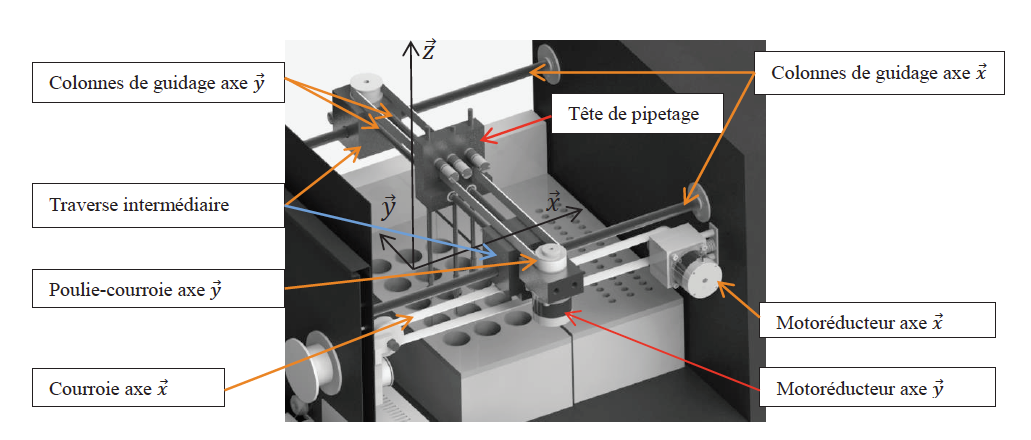
\includegraphics[width=1.0\linewidth]{schema_axez}
\end{marginfigure}
%	%\caption{Diagramme de bloc interne et présentation de l'architecture du système de mesure et du système de guidage \label{chronometrie_IBD}}
%%\end{figure}


\subsection*{Réglage de l'asservissement}


La modélisation de l'asservissement de position est donnée par le schéma-bloc ci-dessous dans lequel $K_2 = 2,78 \cdot 10^{-2} \text{N}^{-1}$, $K_1 = \SI{856}{s^{-1}}$, $T_m= 3\cdot  10^{-2} s$.

Le couple résistant $C_r$ est constant et vaut $C_{r0} = 2,7 \cdot 10^{-3} \text{Nm}$.



\begin{marginfigure}
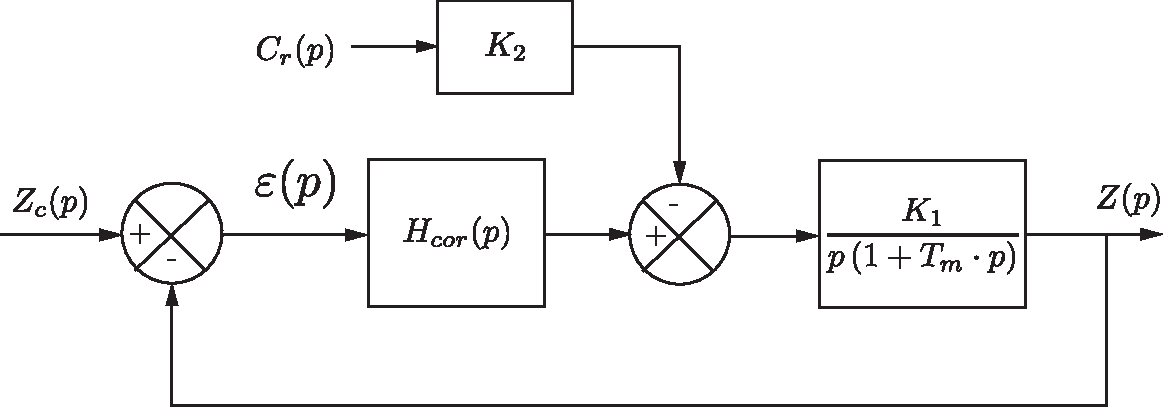
\includegraphics[width=\linewidth]{schema_bloc.pdf}
\end{marginfigure}

On suppose le correcteur proportionnel : $\indice{H}{cor}(p)=K_p$.

Les performances du système sont détaillées dans le diagramme des exigences partiel.% (figure \ref{req}). 


%\begin{figure}[h!]
	\begin{marginfigure}
			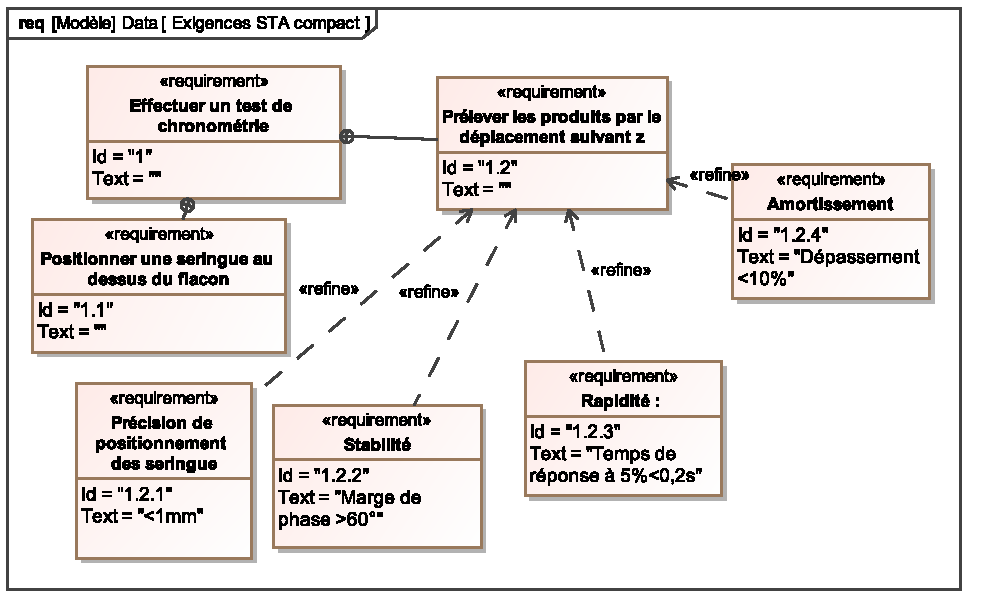
\includegraphics[width=1.0\linewidth]{req.pdf}
    \end{marginfigure}
	%\caption{Diagramme des exigences \label{req}}
%\end{figure}


\question{Déterminer l'expression de la fonction de transfert en boucle ouverte $H_{bo}(p)=\left(\frac{Z(p)}{\varepsilon(p)}\right)_{C_r(p)=0}$ ainsi que la fonction de transfert $H_{cr}(p)=\left(\frac{Z(p)}{C_r(p)}\right)_{Z_c=0}$
.}

\question{Déterminer l'erreur statique pour une entrée de type échelon d'amplitude $Z_{c0}$ dans l'hypothèse d'une perturbation nulle ($C_{r0}$). Déterminer ensuite l'erreur due à une perturbation constante $C_{r0}$, dans le cas d'une
consigne de position nulle ($Z_c=0$). En déduire la valeur de $K_p$ pour satisfaire le critère de précision du cahier des charges.}


\question{Sur le document réponse %de la figure (\ref{bode_bo}) 
compléter les diagrammes de Bode en gain et en phase de $H_{bo}(p)$ pour $K_p$ déterminé précédemment. Indiquer si le critère de stabilité est satisfait en justifiant votre démarche par des tracés nécessaires.}

Afin d'améliorer le comportement, on implante un correcteur Proportionnel Intégral ayant pour fonction de transfert : $H_{cor}(p)=\frac{K_p\left(1+T_i\cdot p\right)}{T_i\cdot p}$ avec $K_p=1$ et $T_i = \SI{1}{s}$.

\question{Tracer le diagramme de Bode de la fonction de transfert en boucle ouverte avec ce correcteur avec $K_p=1$ et $T_i = \SI{1}{s}$.}% sur la figure \ref{bode_bo_PI}.}

\question{On souhaite une marge de phase d'au moins $60^{\circ}$. Proposer un réglage de $K_p$ pour satisfaire au cahier des charges.}% Justifier vos calculs par les tracés nécessaires sur la figure \ref{bode_bo_PI}.}

\question{La figure suivante %\ref{reponse_2nd_ordre} 
donne la réponse à un échelon de position de \SI{50}{mm} avec trois types de correcteurs. Vérifier qu'elle est conforme au cahier des charges. Justifier clairement vos réponses en donnant les valeurs numériques pour chaque critère.}


%\begin{figure}[!htb]
\begin{marginfigure}
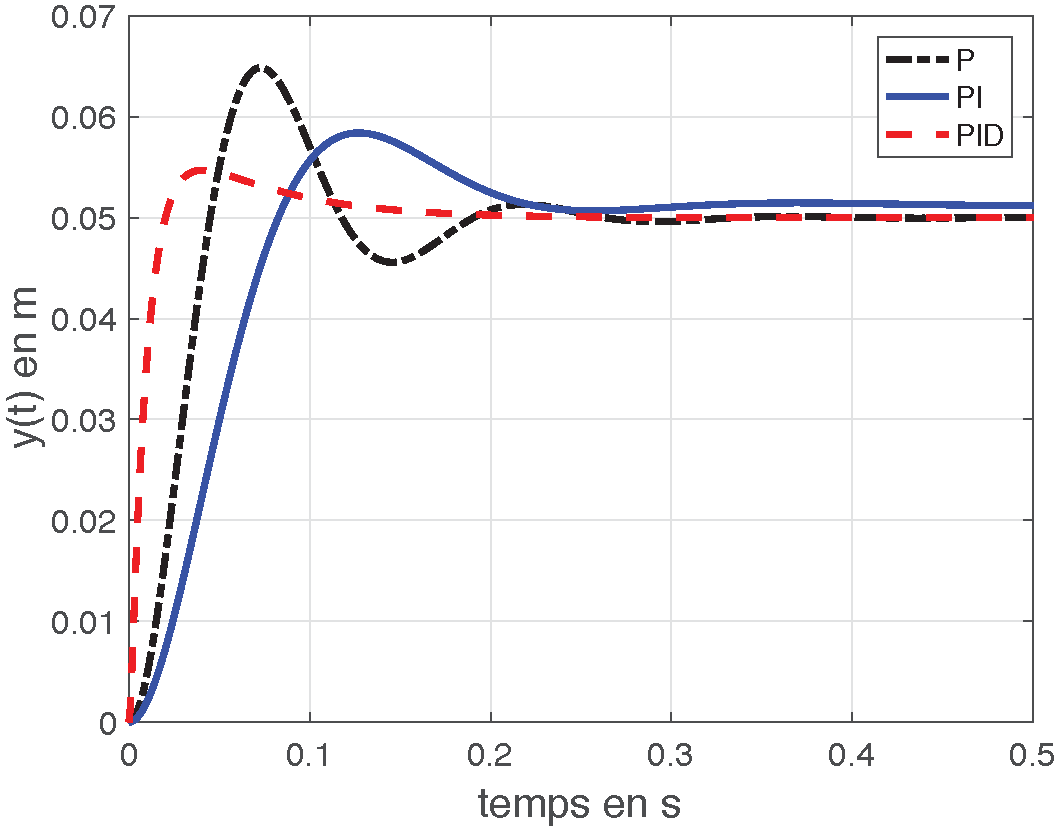
\includegraphics[width=1.0\linewidth]{matlab/rep_temp.pdf}
%\caption{Réponse à un échelon de position de $50 mm$ avec trois correcteurs P(question 2) PI (question 5) et PID (déterminé numériquement)\label{reponse_2nd_ordre}}
\end{marginfigure}
%\end{figure}


\question{Analyser les résultats à l'aide du diagramme de Bode de la FTBO corrigé avec un PID optimisé.}% (figure \ref{bode_pid}.)}

%\begin{figure}[!htb]
\begin{marginfigure}
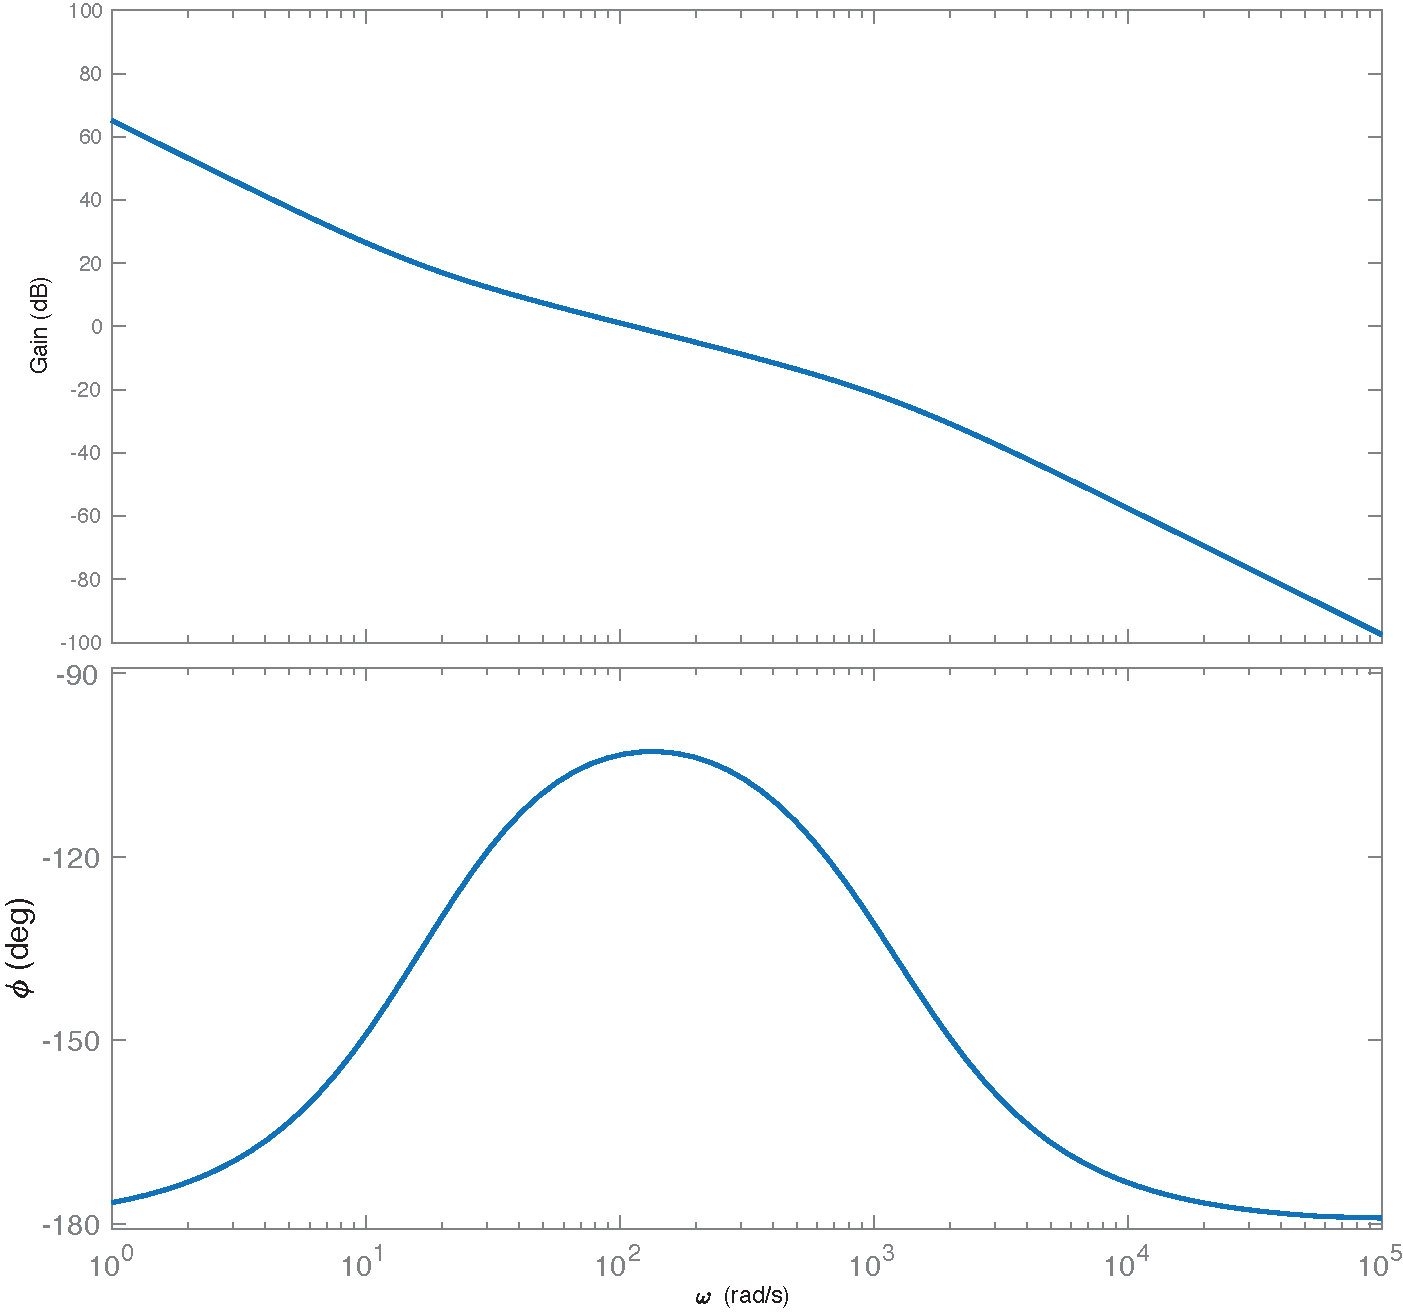
\includegraphics[width=1.0\linewidth]{matlab/bode_pid.pdf}
%\caption{Diagramme de Bode de $H_{bo}(p)$ avec un correcteur PID pour $K_p=0,19$, $K_i=2,1$ et $K_d=0,0038$\label{bode_pid}}
\end{marginfigure}
%\end{figure}


%\begin{figure}[!htb]
\begin{figure}[!h]
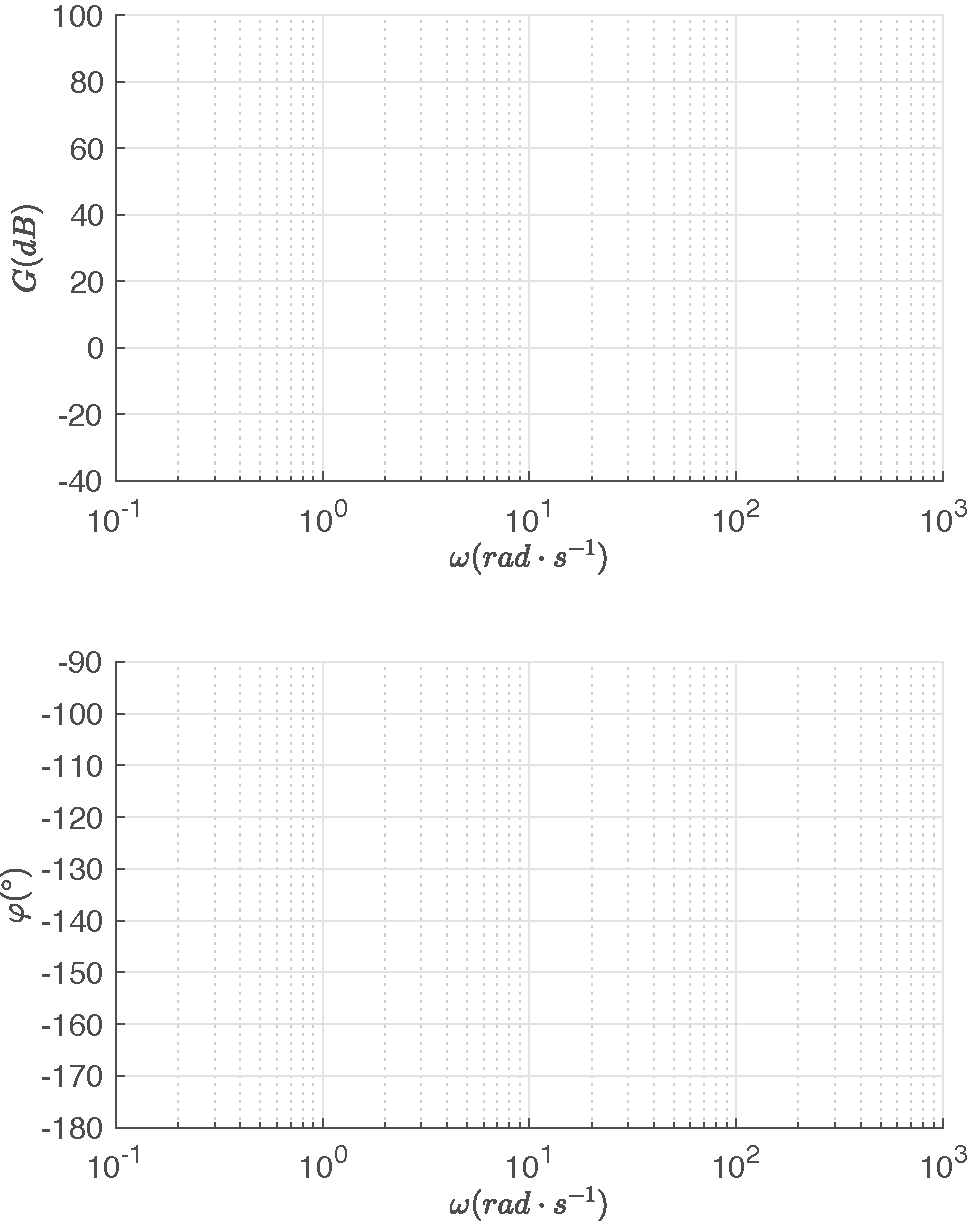
\includegraphics[width=.48\linewidth]{matlab/bode_total0.pdf}
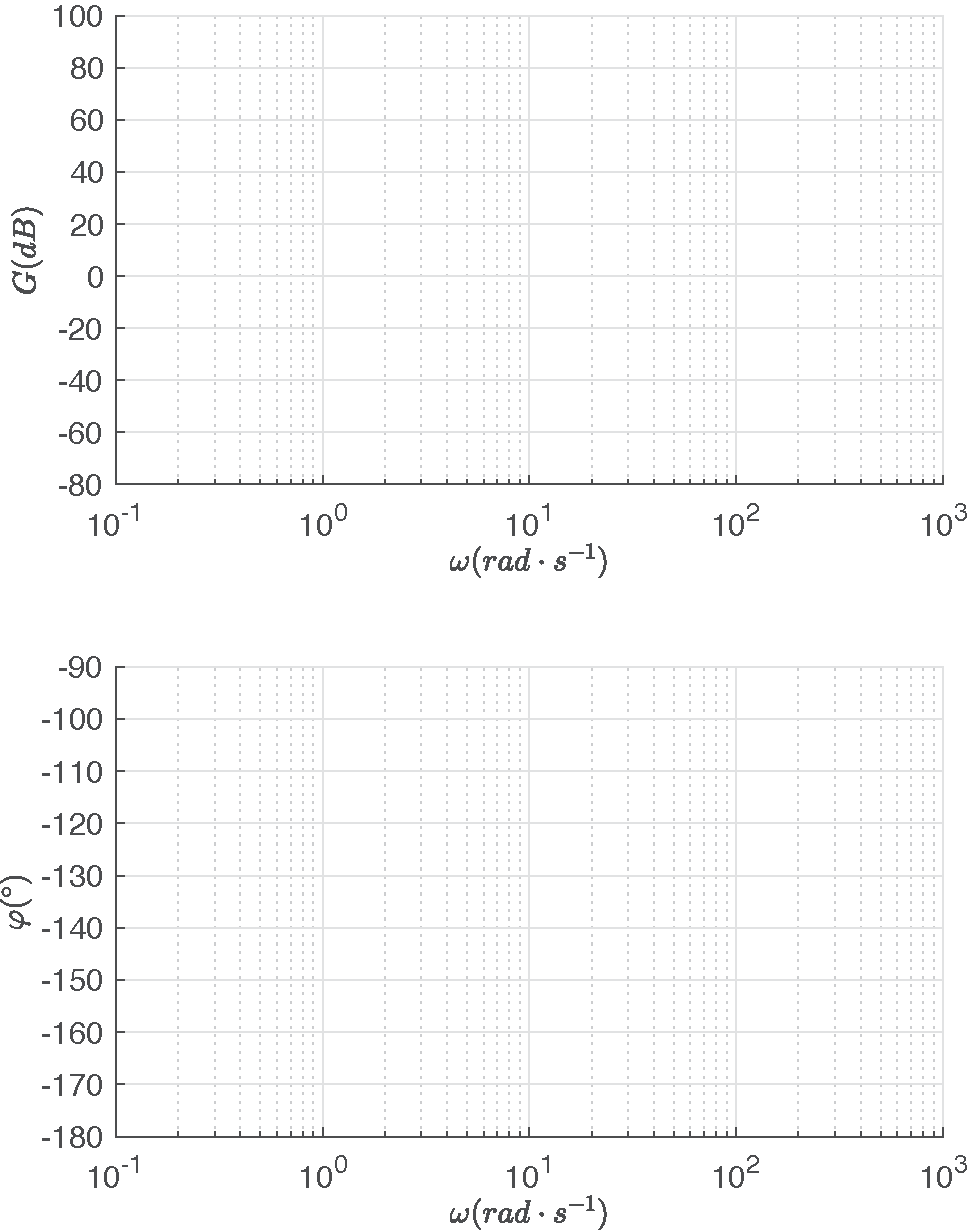
\includegraphics[width=.48\linewidth]{matlab/bode_total0_pi.pdf}
\end{figure}
%\end{figure}
%
%%\begin{figure}[!htb]
%\begin{center}
%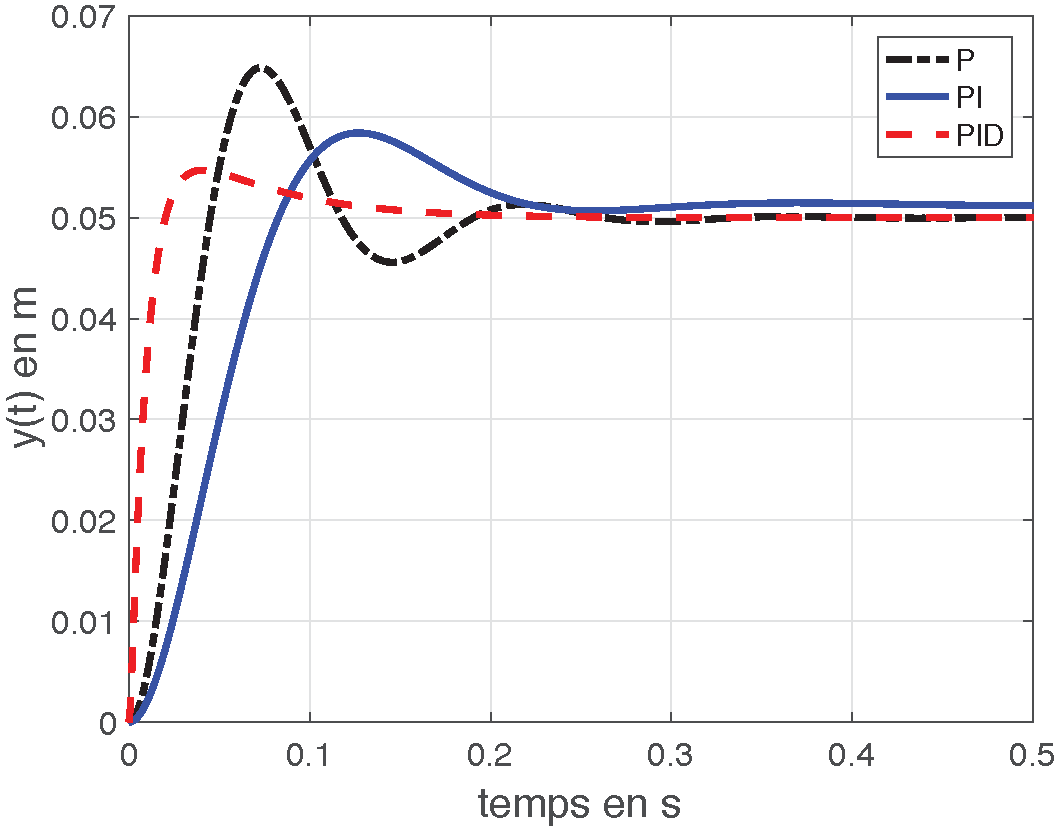
\includegraphics[width=1.0\linewidth]{matlab/rep_temp.pdf}
%%\caption{Réponse à un échelon de position de $50 mm$ avec trois correcteurs P(question 2) PI (question 5) et PID (déterminé numériquement)\label{reponse_2nd_ordre}}
%\end{center}
%%\end{figure}




\ifprof
\newpage

\question{}%sDéterminer l'expression de la fonction de transfert en boucle ouverte $H_{bo}(p)=\left(\frac{Z(p)}{\varepsilon(p)}\right)_{C_r(p)=0}$ ainsi que la fonction de transfert $H_{cr}(p)=\left(\frac{Z(p)}{C_r(p)}\right)_{Z_c=0}$
%.}


${H_{bo}}(p) = \frac{{Z(p)}}{{\varepsilon (p)}} = {H_{cor}}(p)\frac{{{K_1}}}{{p(1 + {T_m}p)}} = \frac{{{K_p}{K_1}}}{{p(1 + {T_m}p)}}$
et $Z(p) = \frac{{{K_1}}}{{p(1 + {T_m}p)}}\left[ {{K_p}\varepsilon (p) - {K_2}{C_r}(p)} \right] = \frac{{{K_1}}}{{p(1 + {T_m}p)}}\left[ {{K_p}( - Z(p)) - {K_2}{C_r}(p)} \right]$
$\Leftrightarrow 
Z(p)(1 + \frac{{{K_p}{K_1}}}{{p(1 + {T_m}p)}}) =  - \frac{{{K_1}{K_2}}}{{p(1 + {T_m}p)}}{C_r}(p)$
$\Leftrightarrow 
{H_{cr}}(p) = {\left( {\frac{{Z(p)}}{{{c_r}(p)}}} \right)_{Zc = 0}} = \frac{{ - \frac{{{K_1}{K_2}}}{{p(1 + {T_m}p)}}}}{{(1 + \frac{{{K_p}{K_1}}}{{p(1 + {T_m}p)}})}} =  - \frac{{{K_1}{K_2}}}{{p(1 + {T_m}p) + {K_p}{K_1}}} =  - \frac{{\frac{{{K_2}}}{{{K_p}}}}}{{1 + \frac{{p(1 + {T_m}p)}}{{{K_p}{K_1}}}}}$.

\question{}%Déterminer l'erreur statique pour une entrée de type échelon d'amplitude $Z_{c0}$ dans l'hypothèse d'une perturbation nulle ($C_{r0}$). Déterminer ensuite l'erreur due à une perturbation constante $C_{r0}$, dans le cas d'une
%consigne de position nulle ($Z_c=0$). En déduire la valeur de $K_p$ pour satisfaire le critère de précision du cahier des charges.}

L'erreur statique par rapport  à une entrée échelon, la perturbation étant nulle, est égale à 0, car il y a une intégration dans la chaine directe

Dans le cas d'une perturbation constante égale à $C_{ro}$, d'après la question précédente on peut écrire :  
$
Z(p) =  - \frac{{\frac{{{K_2}}}{{{K_p}}}}}{{1 + \frac{{p(1 + {T_m}p)}}{{{K_p}{K_1}}}}}{c_r}(p) = - \frac{{\frac{{{K_2}}}{{{K_p}}}}}{{1 + \frac{{p(1 + {T_m}p)}}{{{K_p}{K_1}}}}}\frac{{{C_{ro}}}}{p}$.

En utilisant la propriété du gain statique, on en déduit ${z_\infty } =  \frac{{{K_2}{C_{ro}}}}{{{K_p}}}\,$ , l'erreur vaut donc  $\varepsilon  =  -{z_\infty }= \frac{{{K_2}{C_{ro}}}}{{{K_p}}}\,$.

Pour répondre à l'exigence de précision, on doit avoir $\varepsilon  = \frac{{{K_2}{C_{ro}}}}{{{K_p}}}\, < 1\,mm$.

On en déduit $
\varepsilon  =  \frac{{{K_2}{C_{ro}}}}{{{K_p}}}\, < {10^{ - 3}}\,m\\$
$\Leftrightarrow {K_p} > \frac{{{K_2}{C_{ro}}}}{{{{10}^{ - 3}}}}$
$\Leftrightarrow {K_p} > \frac{{{{2,78.10}^{ - 2}}{{.2,3.10}^{ - 3}}}}{{{{10}^{ - 3}}}}$
$\Leftrightarrow 
{K_p} > 0,075$.




\question{}%Sur le document réponse compléter les diagrammes de Bode en gain et en phase de $H_{bo}(p)$ pour $K_p$ déterminé précédemment. Indiquer si le critère de stabilité est satisfait en justifiant votre démarche par des tracés nécessaires.}

Avec $K_p=0,075$, on obtient une marge de phase de $35^{\circ}<60^{\circ}$, le critère de stabilité n'est donc pas vérifié.

\begin{center}
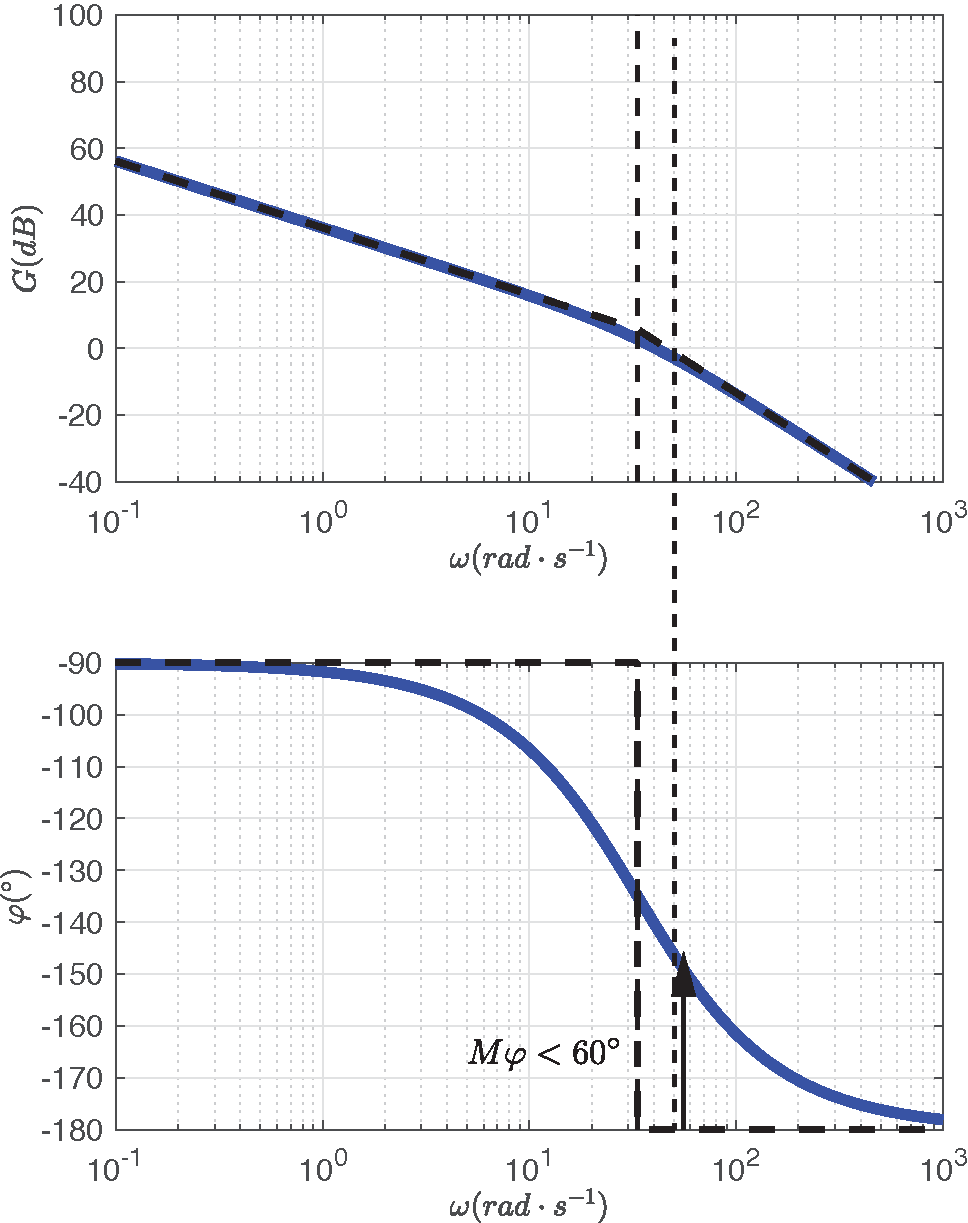
\includegraphics[width=1.0\linewidth]{matlab/bode_total.pdf}
\end{center}

\subparagraph{}%\textit{Tracer le diagramme de Bode de la fonction de transfert en boucle ouverte avec ce correcteur avec $K_p=1$ et $T_i = 1 s$ sur la figure \ref{bode_bo_PI}.}

\begin{center}
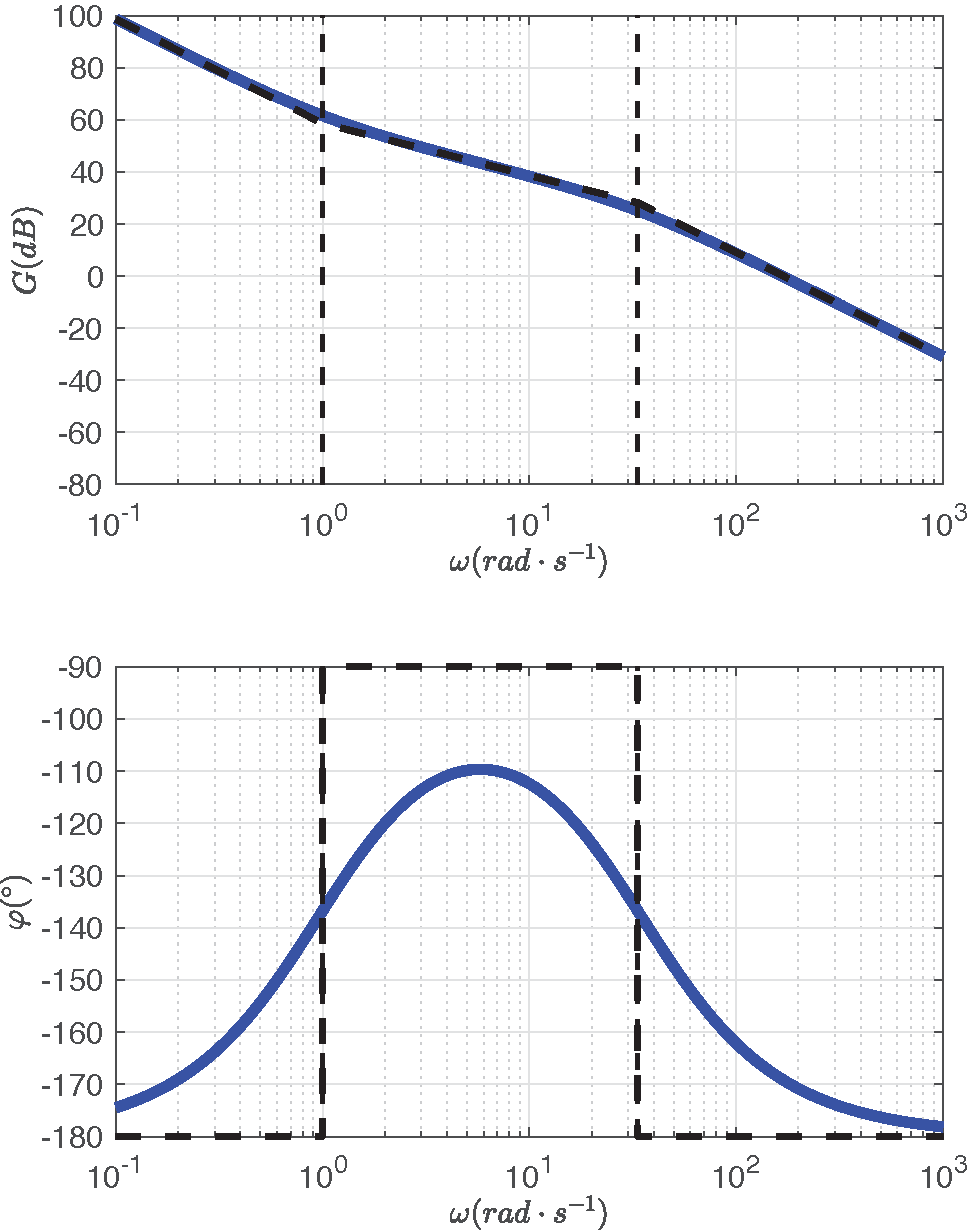
\includegraphics[width=1.0\linewidth]{matlab/bode_total_pi.pdf}
\end{center}

\question{}%On souhaite une marge de phase d'au moins $60^{\circ}$. Proposer un réglage de $K_p$ pour satisfaire au cahier des charges. Justifier vos calculs par les tracés nécessaires sur le diagramme.}% sur la figure \ref{bode_bo_PI}.}

On note qu'en la pulsation donnant une phase à $-120^{\circ}$, le gain en décibel est à peu prêt égal à $-30dB$. On règle donc $K_p$ tel que :

\begin{align*}
\boxed{
K_p=10^{-30/20}=0,032.
}
\end{align*}

On obtient alors le deuxième tracé.

\begin{center}
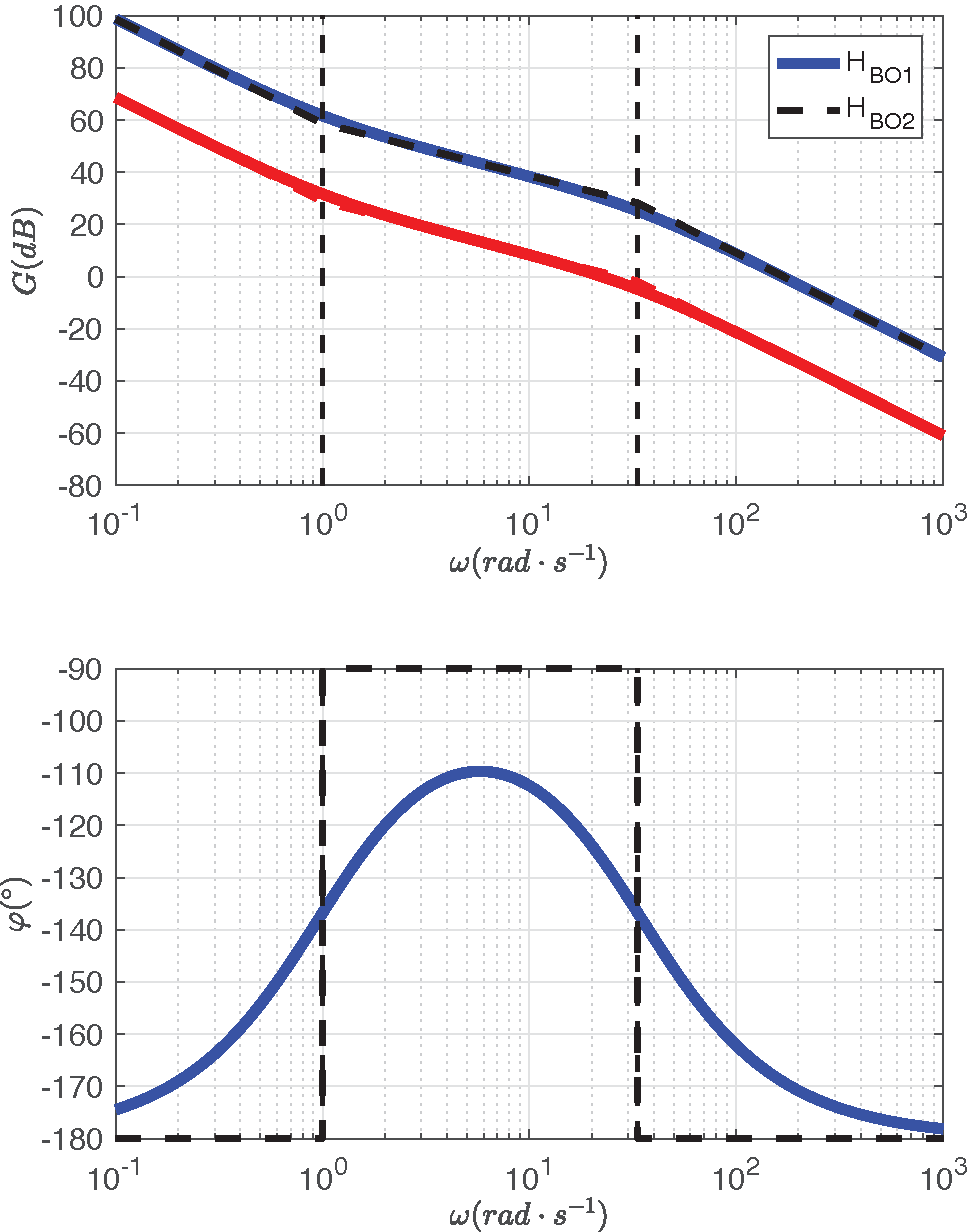
\includegraphics[width=.80\linewidth]{matlab/bode_total3.pdf}
\end{center} 


\question{}%La figure \ref{reponse_2nd_ordre} donne la réponse à un échelon de position de $50 mm$ avec trois types de correcteurs. Vérifier qu'elle est conforme au cahier des charges. Justifier clairement vos réponses en donnant les valeurs numériques pour chaque critère.}

\begin{itemize}
\item La valeur en régime permanent vaut $50mm$ pour les trois réponses, l'erreur statique est nulle le critère de précision
est respecté pour les trois réglages.

\item Temps de réponse à $5\%$ et dépassement : 

\begin{tabular}{|c|c|c|c|}
\hline 
Type de correcteur & \textbf{P} & \textbf{PI} & \textbf{PID} \\ 
\hline 
$tr_{5\%}$ & $0,17s$ & $0,2s$ & $0,08$ \\ 
\hline 
Dépassement & $29,72\%$ & $16,8\%$ & $9,4\%$ \\ 
\hline 
\end{tabular} 

\item Seul le PID vérifie le critère sur le premier dépassement car $D_{1\%}=9,4\%<10\%$. Le critère d'amortissement est
donc respecté.
\end{itemize}

\begin{center}
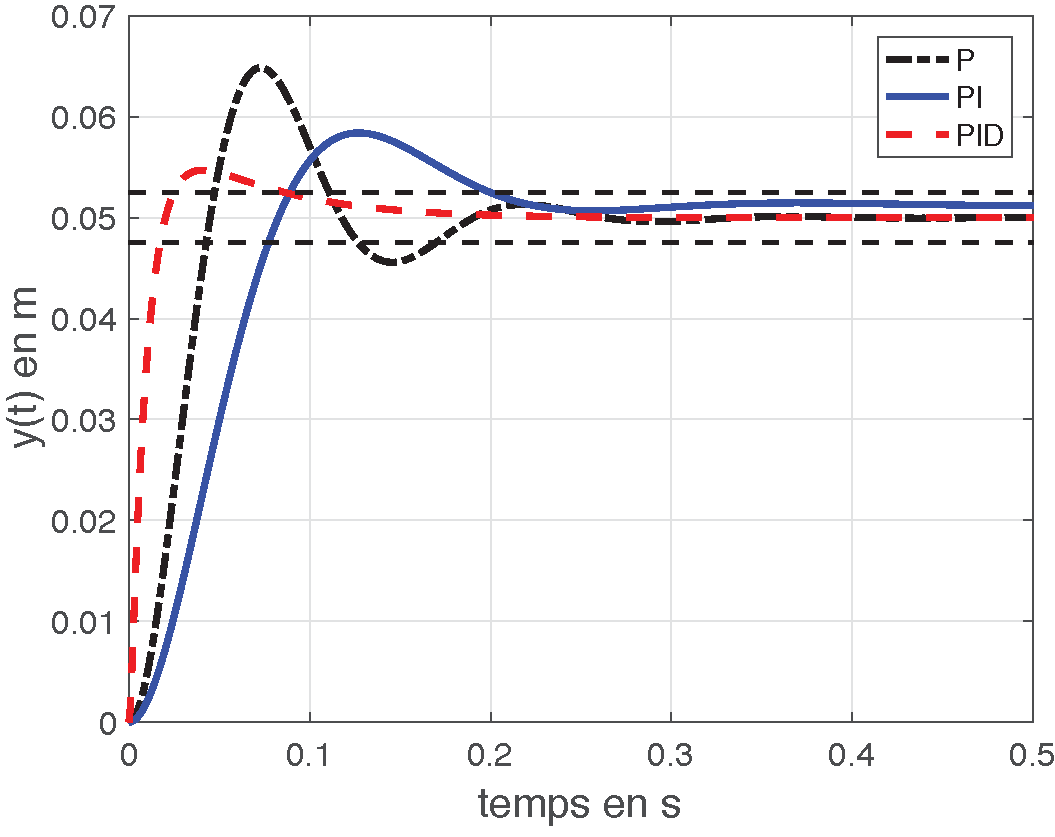
\includegraphics[width=0.7\linewidth]{matlab/rep_temp_corrige.pdf}
\end{center}

\question{}%Analyser les résultats à l'aide du diagramme de Bode de la FTBO corrigé avec un PID optimisé (figure \ref{bode_pid}.)}

On trouve une marge de phase supérieure à $60^{\circ}$ et une bande passante à $0dB$ égale à $100rad/s$ supérieure aux réglages précédents ce qui donne une réponse plus rapide et plus stable.

\else

\fi


\ifprof
\else
\begin{marginfigure}
\centering

\includegraphics[width=3cm]{Cy_03_01_TD_PI_05_Chronometrie_qr}
\end{marginfigure}
\fi
